\documentclass[journal]{IEEEtran}

\usepackage[utf8]{inputenc}
\usepackage{graphicx}
\usepackage{amsmath}
\usepackage{amssymb}
\usepackage{url}
\usepackage{booktabs}
\usepackage{xcolor}
\usepackage{hyperref}
\usepackage{tikz}
\usetikzlibrary{arrows.meta,positioning,fit}

\begin{document}

\title{Mitigating Prompt Injection Attacks in LLM-Based Systems Using Multi-Layer Guardrails: Part II -- Low-Level Design and ML-Backed Validation}

\author{
    \IEEEauthorblockN{Your Name}
    \IEEEauthorblockA{\textit{Your Department} \\
    \textit{Your University or Organization}\\
    City, Country \\
    your.email@example.com}
}

\maketitle
\setcounter{page}{6}

\begin{abstract}
This second part documents the low-level design of Gradril. It maps the architecture to actual extension and back-end modules, details the local validators, explains sanitizer behavior, and describes the currently implemented ML-backed Guardrails services and the optional semantic detector endpoint. It also clarifies the current runtime behavior of the decision engine, which performs allow-or-sanitize actions rather than hard local blocking.
\end{abstract}

\begin{IEEEkeywords}
LLM security, low-level design, ML validation, Guardrails AI, semantic detector.
\end{IEEEkeywords}

\section{Low-Level Design}
The implemented prototype consists of a TypeScript Visual Studio Code extension and a Python validation service. The extension is responsible for prompt interception, local validation, sanitization, audit logging, and user feedback. The Python service hosts Guardrails-based input and output checks and a separate semantic similarity endpoint.

\begin{figure}[ht]
\centering
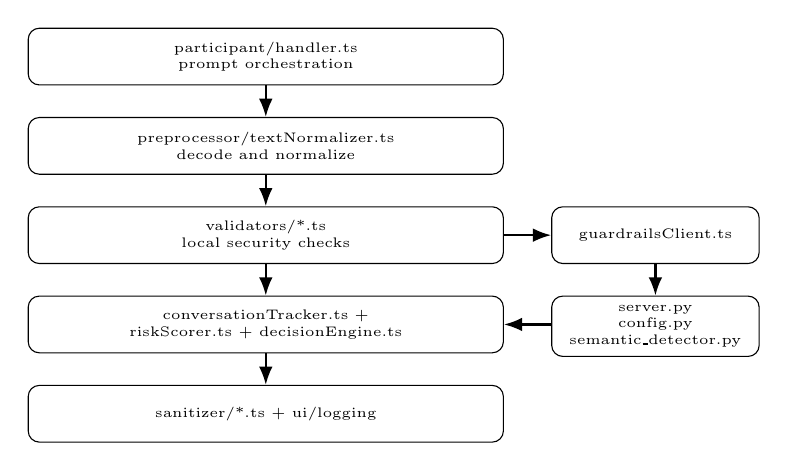
\begin{tikzpicture}[
    font=\tiny,
    node distance=4mm,
    box/.style={draw, rounded corners, align=center, text width=5.8cm, minimum height=0.72cm},
    side/.style={draw, rounded corners, align=center, text width=2.4cm, minimum height=0.72cm},
    line/.style={-Latex, thick}
]
\node[box] (handler) {participant/handler.ts\\prompt orchestration};
\node[box, below=of handler] (norm) {preprocessor/textNormalizer.ts\\decode and normalize};
\node[box, below=of norm] (validators) {validators/*.ts\\local security checks};
\node[box, below=of validators] (engine) {conversationTracker.ts + riskScorer.ts + decisionEngine.ts};
\node[box, below=of engine] (sanitize) {sanitizer/*.ts + ui/logging};
\node[side, right=6mm of validators] (client) {guardrailsClient.ts};
\node[side, below=of client] (backend) {server.py\\config.py\\semantic\_detector.py};
\draw[line] (handler) -- (norm);
\draw[line] (norm) -- (validators);
\draw[line] (validators) -- (engine);
\draw[line] (engine) -- (sanitize);
\draw[line] (validators.east) -- (client.west);
\draw[line] (client) -- (backend);
\draw[line] (backend.west) |- (engine.east);
\end{tikzpicture}
\caption{Low-level implementation view.}
\end{figure}

\section{Local Validators}
The extension currently registers seven validators in code:
\begin{enumerate}
    \item PII detector,
    \item secret detector,
    \item injection detector,
    \item jailbreak detector,
    \item toxicity detector,
    \item code exfiltration detector,
    \item multi-turn conversation tracker.
\end{enumerate}

However, only five are enabled by default in the current configuration: PII, secrets, injection, jailbreak, and toxicity. The code exfiltration and multi-turn modules are implemented but not default-active unless settings are extended.

\subsection{PII and Secret Detection}
The PII detector targets e-mail addresses, phone numbers, credit-card patterns, dates of birth, IP addresses, and related identifiers. The secret detector targets API keys, tokens, connection strings, private keys, and password-like assignments. These are primarily regex and heuristic based on the extension side.

\subsection{Injection and Jailbreak Detection}
The injection detector focuses on instruction override, role hijack, prompt extraction, delimiter injection, meta-instructions, and related manipulation patterns. The jailbreak detector extends this set with role-play escalation, named jailbreak families, encoding-evasion hints, refusal suppression, and prompt-framing attacks.

\subsection{Code Exfiltration and Multi-Turn Detection}
The code exfiltration detector looks for attempts to induce generation of scripts that print environment variables, read credential files, serialize secrets, or send data over a network. The conversation tracker stores recent prompt context and looks for staged or split attacks across multiple turns.

\section{Sanitization and Decision Logic}
The local decision engine returns only two actions: \texttt{ALLOW} and \texttt{SANITIZE}. When findings are present, the prompt is sanitized and forwarded rather than blocked. PII and secrets are masked with placeholders. Injection-related findings are stripped. This design choice makes Gradril a sanitize-or-pass guardrail rather than a hard prompt firewall.

\section{Back-End Input and Output Guards}
The Python back end defines two Guardrails configurations.

\subsection{Input Guard}
The input guard applies:
\begin{itemize}
    \item \texttt{DetectPII} -- \texttt{on\_fail=fix}
    \item \texttt{ToxicLanguage} -- \texttt{on\_fail=exception}
    \item \texttt{DetectJailbreak} -- \texttt{on\_fail=exception}
    \item \texttt{SecretsPresent} -- \texttt{on\_fail=fix}
    \item \texttt{UnusualPrompt} -- \texttt{on\_fail=noop}
\end{itemize}

\subsection{Output Guard}
The output guard applies:
\begin{itemize}
    \item \texttt{GroundedAIHallucination} -- \texttt{on\_fail=noop}
    \item \texttt{BiasCheck} -- \texttt{on\_fail=noop}
    \item \texttt{ToxicLanguage} -- \texttt{on\_fail=exception}
    \item \texttt{DetectPII} -- \texttt{on\_fail=fix}
\end{itemize}

\section{ML Models and Engines}
The project documentation and configuration identify the following ML-backed engines:
\begin{table}[ht]
\centering
\caption{ML models and engines used or referenced by Gradril}
\begin{tabular}{p{2.2cm}p{4.4cm}}
\toprule
\textbf{Validator} & \textbf{Model / Engine} \\ \midrule
DetectPII & Microsoft Presidio + spaCy \texttt{en\_core\_web\_lg} \\
ToxicLanguage & \texttt{unitary/toxic-bert} \\
DetectJailbreak & Guardrails jailbreak detector \\
GroundedAIHallucination & GroundedAI model \\
BiasCheck & \texttt{d4data/bias-detection-model} \\
Semantic detector & \texttt{sentence-transformers/all-MiniLM-L6-v2} \\ \bottomrule
\end{tabular}
\end{table}

\section{Optional Semantic Endpoint}
The repository includes a dedicated semantic detector implemented in \texttt{semantic\_detector.py}. It embeds prompts and malicious prototypes using sentence-transformers and scores similarity through cosine distance. This is a meaningful research contribution, but it is not yet connected to the active extension request path. Accordingly, it should be presented as an implemented extension capability rather than a fully deployed runtime component.

\section{Output-Validation Limitation}
A practical implementation detail is that output validation occurs after generation. Therefore hallucination, bias, toxicity, or PII findings on the output side primarily support annotation or redaction rather than pre-display enforcement. This should be stated clearly in any final research manuscript.

\section{Conclusion of Part II}
Part II described the concrete implementation of the Gradril prototype, including local validators, sanitizer behavior, decision logic, Guardrails back-end services, and the optional semantic detector. Part III covers the evaluation protocol, benchmark design, baselines, and publication-ready experimental framing.

\end{document}
